\section{Complexity}

\begin{figure}[p]
    \centering
    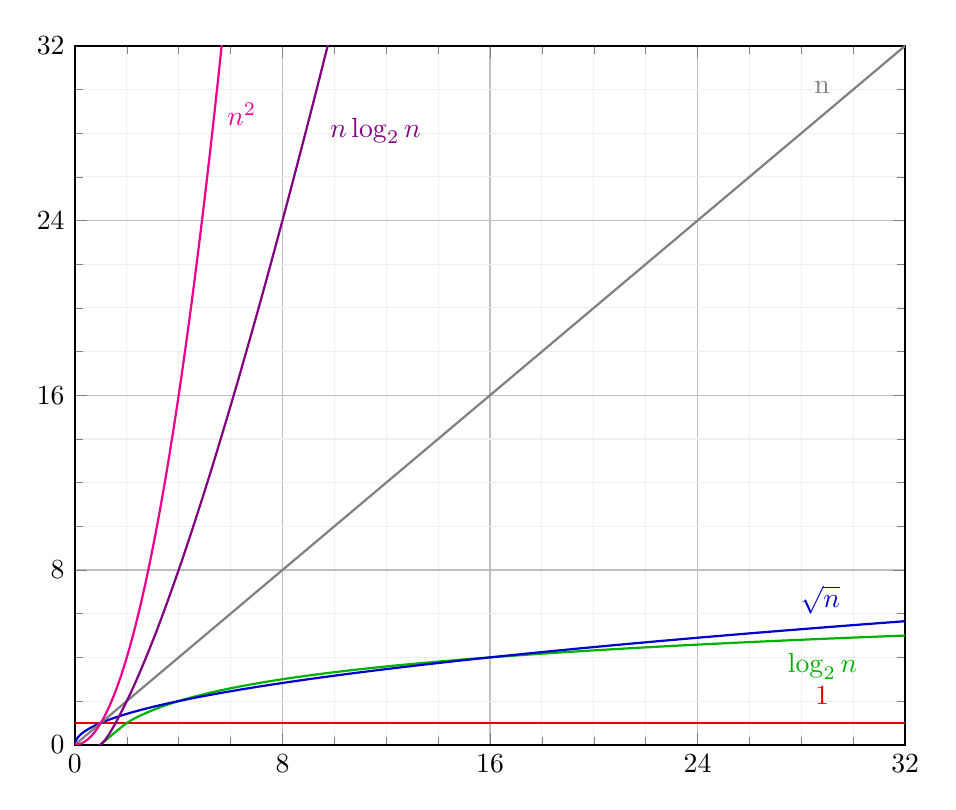
\begin{tikzpicture}
    \begin{axis}[
        width = \hsize, thick, smooth,
        domain = 0:32, xmin = 0, xmax = 32, ymin = 0, ymax = 32,
        xtick distance = 8, ytick distance = 8,
        minor tick num = 3,
        grid = both,
        major grid style = {lightgray},
        minor grid style = {lightgray!25},
        legend cell align = left,
    ]
        \addplot[red!90!black] {1}
            [yshift=1em] node [pos=0.9] {1};
        \addplot[green!70!black, samples = 32] {log2(x)}
            [yshift=-1em] node [pos=0.9] {$\log_{2}n$};
        \addplot[blue!80!black, samples = 512] {sqrt(x)}
            [yshift=1em] node [pos=0.9] {$\sqrt{n}$};
        \addplot[gray] {x}
            [yshift=1em] node [pos=0.9] {n};
        \addplot[violet, samples = 32] {x * log2(x)}
            [xshift=2em,yshift=-2em] node [pos=0.2] {$n \log_{2}n$};
        \addplot[magenta, samples = 128] {x * x}
            [xshift=1em] node [pos=0.029] {$n^2$};
    \end{axis}
\end{tikzpicture}

    \caption{Algorithmic complexity functions}
    \label{fig:algo:comp}
\end{figure}

The single most important graph in algorithmic complexity analysis is shown in
figure \ref{fig:algo:comp}.  The values of different functions are shown for
increasing positive values of the variable $n$.  These functions are used to
describe the relationship between an algorithm's resource consumption (for any
given resource of interest: number of operations/instructions, memory/disk
storage, etc.) and the size of its input.

The complexity of an algorithm is also called its \textit{order}, and the formal
definition of algorithmic complexity uses what is for that reason called
\textit{Big Omicron} or \textit{Big O} notation\footnotemark, which has the form
$f \in O(g)$.  It describes the relation between the complexity function $f$ of
an algorithm and a function $g$ according to the following principles:

\footnotetext{
    The former being a later rechristening based on Knuth's use of
    $\omega$/$\Omega$ (small omega / big omega).}

\begin{itemize}
    \item
        The notation is asymptotic: $f \in O(g)$ implies that $g$ is an upper
        bound for $f$: $f(n) <= g(n)$ for some range of values.
    \item Input sizes are always positive real numbers: $0 <= n$.
    \item
        The analysis is primarily focused on large input sizes.  Some orders may
        be faster for smaller sizes, but those are rarely the important parts of
        a program.  Therefore, $f \in O(g)$ if there is a value $n_0$ for which
        $f(n) <= g(n)$ for all $n_0 < n$, that is, even if $g(n) <= f(n)$ for
        some values of $n$, provided there is a point after which $g$ is always
        an upper bound for $f$.
    \item
        Similarly, differences between machines are critical factors but very
        difficult to analyze in the abstract, so $f \in O(g)$ if there is a
        constant $c > 0$ for which $c f(x) <= g(x)$.  That is, even if some
        constant factor influences the complexity of a specific implementation
        of an algorithm, it will become irrelevant for large input sizes and can
        be ignored.
    \item
        Usually, only the tightest bound for a function is considered.  E.g.:
        even though it is true that $f \in O(\log{n})$ implies $f \in O(n)$ (but
        not $f \in O(1)$), $O(n)$ usually means $f(n)$ is the most restrictive
        of the categories that fits the constraints above.  In general, for any
        polynomial, only its highest power of $n$ is considered, as it
        eventually dominates the value of the function.
\end{itemize}

Note that these definitions are idealistic: their intent is to formalize the
resource utilization of an algorithm as much as possible across machines of
drastically different characteristics.  As such, they model computation \emph{in
vacuo}, offering only a partial --- if very useful --- characterization
intrinsic to an algorithm, but a complete analysis must consider the
architectural components described in chapter \secref{ch:arch} and elsewhere.

Big O is part of a family of notations which describe relations between
functions.  Table \ref{tbl:algo:big_o} lists those most commonly used in
complexity analysis.

\begin{table}[ht]
    \centering
    \begin{tabular}{ccl}
        Notation & Name & Description (asymptotic) \\
        \hline
        $f(n) \in o(g(n))$ & small O / Omicron & dominated by \\
        $f(n) \in O(g(n))$ & big O / Omicron & bounded above by (see text) \\
        $f(n) \in \Theta(g(n))$ & big Theta & bounded below and above by \\
        $f(n) \sim g(n)$ & order of & equal to \\
        $f(n) \in \Omega(g(n))$ & big Omega & bounded below by \\
        $f(n) \in \omega(g(n))$ & small Omega & dominates \\
    \end{tabular}
    \caption{Family of complexity notations}
    \label{tbl:algo:big_o}
\end{table}

\textit{Constant complexity}, $f(n) = 1$, represents any function that does not
depend on the magnitude of its input.  A hash table lookup is an example of this
complexity: if the load factor of the table is managed, the number of operations
performed is independent of the number of elements in the table.  Even though
this function is usually represented by the constant $1$, from the rules above
we derive that any constant function is in the same category.

\textit{Linear complexity}, $f(n) = n$, is a function directly proportional to
its input.  Algorithms commonly operate on every element, consume one unit of
space, or otherwise perform an operation for each of their input values, making
this the most common function to describe their complexity, and a reference to
which other functions are compared.  A linear search over an array of elements
is an example of this complexity.

Different interesting subsets of these functions can be analyzed in separation
so that the scale of the graphs can be adjusted, as they quickly become wildly
divergent outside the range displayed in the graph.  Figure
\ref{fig:algo:comp_nlog_sqrt_n} compares the lower part of the original graph to
the growth of $n$, this time using a logarithmic scale.

\begin{figure}[ht]
    \centering
    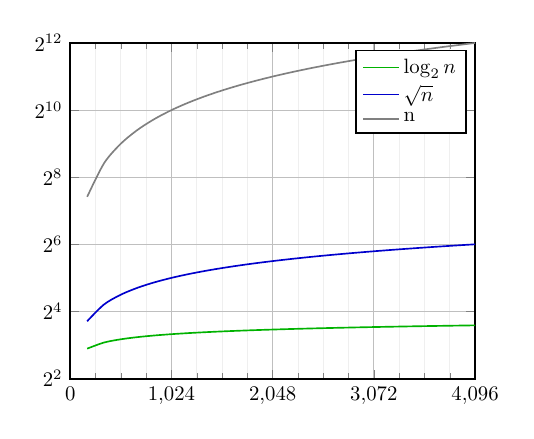
\begin{tikzpicture}[scale=0.75]
        \begin{semilogyaxis}[
            thick, smooth,
            log basis y = 2,
            domain = 0:4096, xmin = 0, xmax = 4096, ymax = 4096,
            xtick distance = 1024,
            minor tick num = 3,
            grid = both,
            major grid style = {lightgray},
            minor grid style = {lightgray!25},
            legend cell align = left,
        ]
            \addplot[green!70!black] {log2(x)};
            \addplot[blue!80!black] {sqrt(x)};
            \addplot[gray] {x};
            \legend{$\log_{2}n$, $\sqrt{n}$, n}
        \end{semilogyaxis}
    \end{tikzpicture}
    \caption{$n \log_{2}n$ vs. $\sqrt{n}$}
    \label{fig:algo:comp_nlog_sqrt_n}
\end{figure}

\textit{Logarithmic complexity} (referring as always in this section to the
logarithm base 2 unless given an explicit base), $f(n) = \log_{2}n$, is the
pattern of algorithms that reduce their domain by some constant factor in each
iteration, usually by half.  A binary search is an example of this complexity.

This is a very important function that is common of optimized algorithms which
dramatically reduces resource consumption, as the $\log_{2}$ remains a
relatively low number, very similar to a constant factor, even for very large
(in terms of numbers that computers usually deal with) values of $n$.  As an
example, the two most common word sizes currently are 32 and 64 bits.  These can
address arrays of roughly two million and ten quintillion bytes, but the
logarithm base two of those values is, obviously, 32 and 64.  This demonstrates
both that doubling the logarithm has an enormous effect on the corresponding
value of $n$ and that the logarithm is relatively small for very large values of
$n$.

\textit{Fractional power complexity} is a less common case of algorithms which
reduce their input by a fractional exponent, typically 2 --- i.e. $f(n) =
\sqrt(n)$.  A linear primality test that tests the divisibility by every number
up to the square root of its input is an example of this complexity.  Although
both $n \log_{2}n$ and $\sqrt{n}$ appear lower and very similar in the original
graph, the latter grows more quickly, as can be seen in the logarithmic scale
graph, but both stay several orders of magnitude below $n$.

\textit{Quasilinear complexity}, $f(n) = n \log_{2}n$ is also a common case of
algorithms that reduce their domain by half as in the case of logarithmic
complexity but in relation to the operations performed for each of its input
elements.  Sorting algorithms are an example of this complexity.  Although the
original graph shows this function quickly growing past the range displayed,
this class of algorithms is still considered tractable as, just like for
logarithmic complexity, the logarithm resembles a constant at larger values of
$n$.

Figure \ref{fig:algo:comp_n_nlog} shows the relationship between the functions
$n \log_{2}n$ and $n$.  While steeper, its growth is contained due to the fact
that the $\log_{2}n$ term has a relatively moderate growth, as we saw when we
analyzed logarithmic complexity.

\begin{figure}[ht]
    \centering
    \hfill
    \begin{subfigure}[h]{0.45\textwidth}
        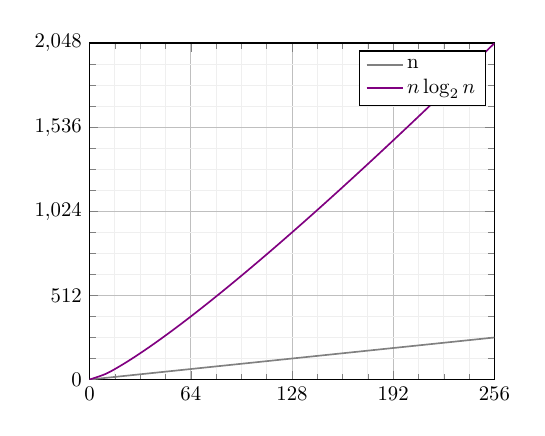
\begin{tikzpicture}[scale=0.75]
            \begin{axis}[
                thick, smooth,
                domain = 0:256, xmin = 0, xmax = 256, ymin = 0, ymax = 2048,
                xtick distance = 64, ytick distance = 512,
                minor tick num = 3,
                grid = both,
                major grid style = {lightgray},
                minor grid style = {lightgray!25},
                legend cell align = left,
            ]
                \addplot[gray] {x};
                \addplot[violet] {x * log2(x)};
                \legend{n, $n \log_{2}n$}
            \end{axis}
        \end{tikzpicture}
        \caption{n vs. $n \log_{2}n$}
        \label{fig:algo:comp_n_nlog}
    \end{subfigure}
    \hfill
    \begin{subfigure}[h]{0.45\textwidth}
        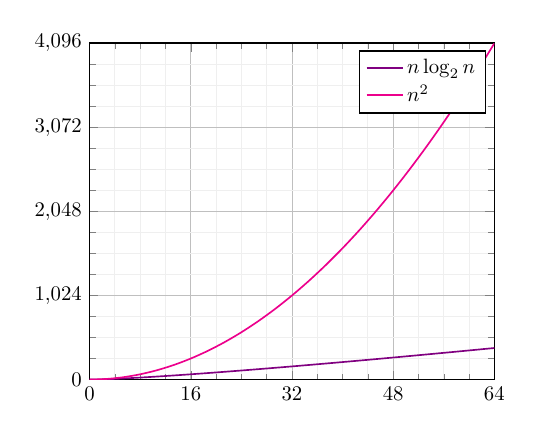
\begin{tikzpicture}[scale=0.75]
            \begin{axis}[
                thick, smooth,
                domain = 0:64, xmin = 0, xmax = 64, ymin = 0, ymax = 4096,
                xtick distance = 16, ytick distance = 1024,
                minor tick num = 3,
                grid = both,
                major grid style = {lightgray},
                minor grid style = {lightgray!25},
                legend cell align = left,
            ]
                \addplot[violet] {x * log2(x)};
                \addplot[magenta] {x * x};
                \legend{$n \log_{2}n$, $n^2$}
            \end{axis}
        \end{tikzpicture}
        \caption{$n \log_{2}n$ vs. $n^2$}
        \label{fig:algo:comp_nlog_n2}
    \end{subfigure}
    \hfill
    \caption{$n, n \log_{2}n, n^2$}
    \label{fig:algo:comp_n_nlog_n2}
\end{figure}

\textit{Polynomial complexity} describes algorithms whose complexity is defined
by a polynomial.  Quadratic complexity, $f(n) = n^2$, is its most common type,
where an algorithm performs an operation for each element of the Cartesian
product of its input.  Less optimized sorting algorithms, such as selection and
bubble sort, are examples of this complexity.

Figure \ref{fig:algo:comp_nlog_n2} shows the relationship between $n \log_{2}n$
and $n^2$.  While both are shown to rise quickly above $n$, the growth of $n^2$
is much more rapid (in a non-linear fashion) compared to $n \log_{2}n$.
